\begin{figure*}
    \centering
    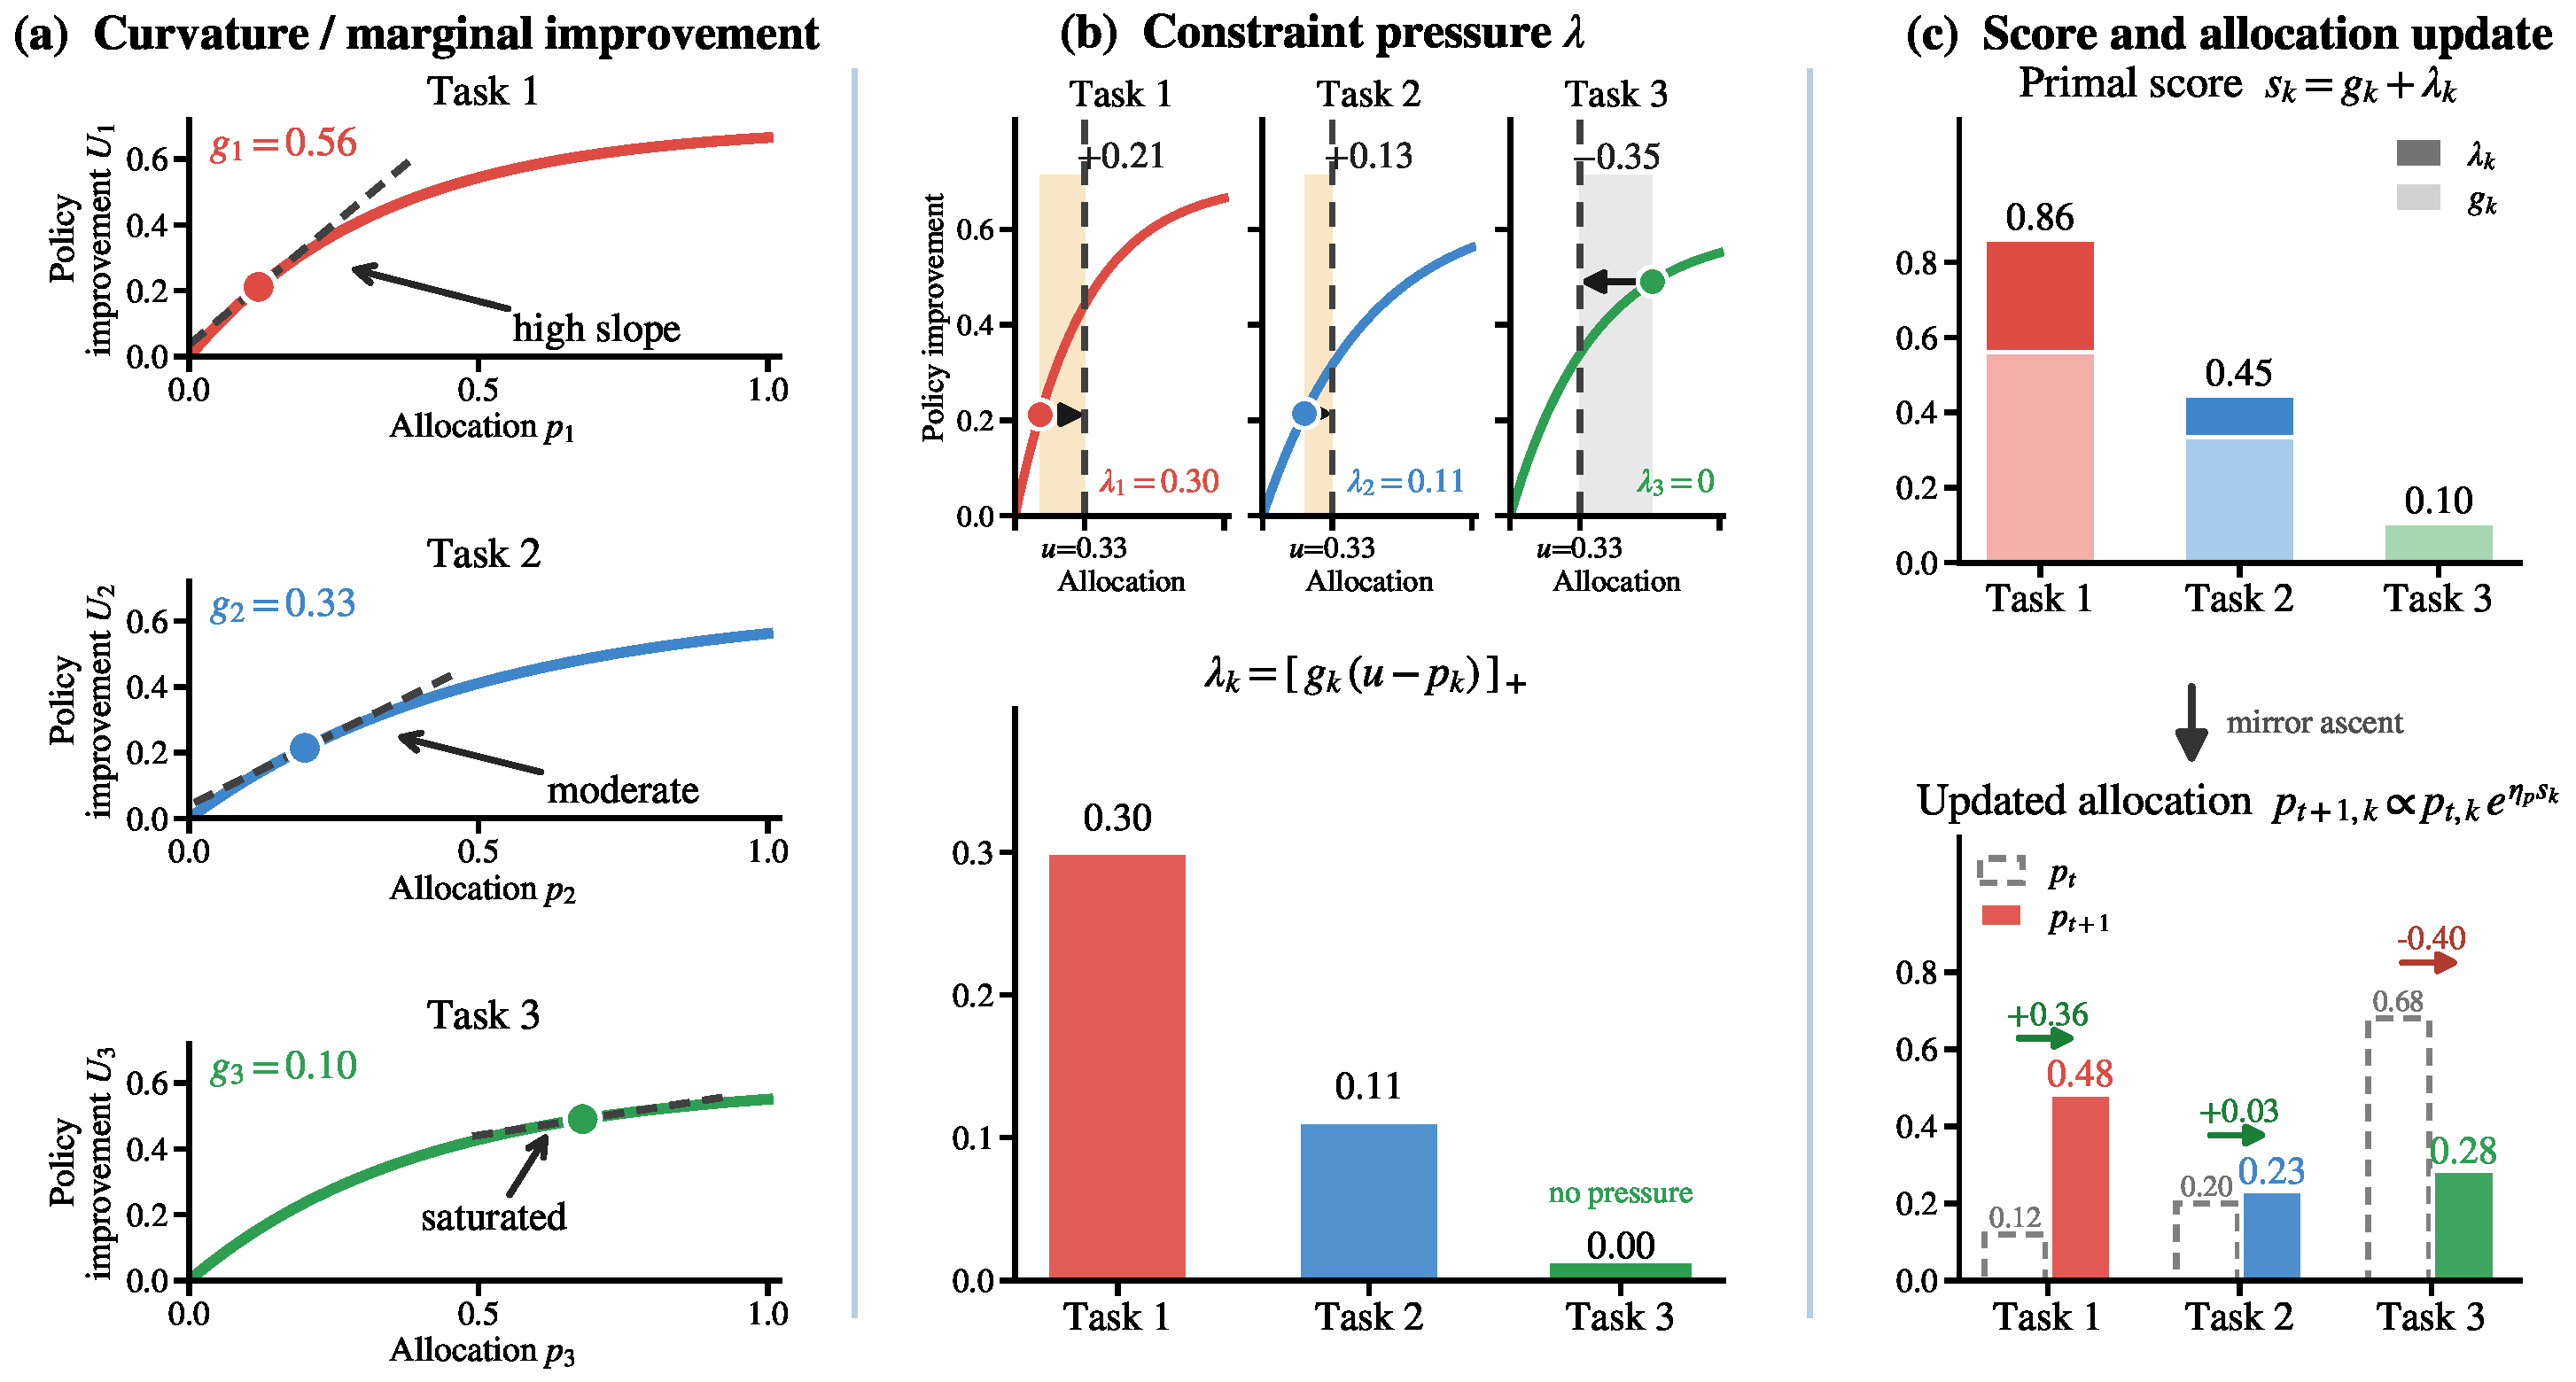
\includegraphics[width=\textwidth]{fig/pdcm_main_fig.pdf}
    \vspace{-\intextsep}
    \caption{%
        \textbf{Curvature-driven allocation in PDCM.}
        \textbf{(a)} Concave policy improvement per task; the slope
        $g_k=\partial U_k/\partial p_k$ at the current allocation gives the marginal
        return (Task~1 steep, Task~3 saturated).
        \textbf{(b)} Constraint pressure as an alignment of the uniform gap with
        curvature, $\lambda_k=[g_k(u-p_k)]_+$, $u=1/K$: only tasks that are both
        under-allocated and still improving accumulate pressure.
        \textbf{(c)} The primal score $s_k=g_k+\lambda_k$ drives the mirror-ascent
        update $p_{t+1,k}\propto p_{t,k}e^{\eta_p s_k}$, moving budget from the
        saturated task to the steep, under-served one.
    }
    \label{fig:pdcm_overview}
    \vspace{-\intextsep}
\end{figure*}